% vim: set spell spelllang=en tw=100 et sw=4 sts=4 :

\documentclass{llncs}

% \usepackage{showframe}

\usepackage{complexity}
\usepackage{hyperref}
\usepackage{microtype}
\usepackage{cleveref}                  % no need to type Figure etc

\usepackage{todonotes}
\usepackage{booktabs}

% lncs style
\crefname{algocf}{Algorithm}{Algorithms}
\Crefname{algocf}{Algorithm}{Algorithms}
\crefname{figure}{Fig.}{Figs.}
\Crefname{figure}{Fig.}{Figs.}
\crefname{table}{Table}{Tables}
\Crefname{table}{Table}{Tables}
\crefname{proposition}{Proposition}{Propositions}
\Crefname{proposition}{Proposition}{Propositions}

\title{Portfolios of Subgraph Isomorphism Algorithms}

\author{
    Lars Kotthoff\inst{1}
    \and Ciaran McCreesh\thanks{This work was supported by the Engineering
        and Physical Sciences Research Council [grant number EP/K503058/1]}\inst{2}
    \and Patrick Prosser\inst{2}
    \and Christine Solnon\inst{3}}

\institute{
    University of British Columbia, Vancouver, Canada
    \and University of Glasgow, Glasgow, Scotland
    \and INSA-Lyon, LIRIS, UMR5205, F-69621, France}

\begin{document}

\maketitle

\begin{abstract}
The subgraph isomorphism problem is a computationally challenging problem with
lots of important practical applications, for example in computer vision,
biochemistry, and model checking. There are a number of state-of-the-art
algorithms for solving it, each of which has its own performance
characteristics. As with many other hard problems, the single best choice of
algorithm overall is rarely the best algorithm for each instance. We develop a
portfolio approach that leverages novel features to characterise subgraph
isomorphism problems to dynamically decide which algorithm to use on a
per-instance basis. We demonstrate significant performance improvements on a
large set of hard benchmark problems. In addition, we show how algorithm
selection models can be leveraged to gain new insights into what affects the
performance of an algorithm.
\end{abstract}

\section{Introduction}

The \emph{(non-induced) subgraph isomorphism problem} is to find an injective mapping from a small
\emph{pattern} graph to a large \emph{target} graph which preserves adjacency. This problem is
\NP-complete, but applications in chemistry and computer vision and model checking and some other
things we should cite mean various exact algorithms exist:

\begin{itemize}
    \item VF2 \cite{Cordella:2004} is a backtracking search algorithm which is especially fast on
        trivially satisfiable instances (which are common in certain application areas).
    \item LAD \cite{Solnon:2010} and SND \cite{Audemard:2014} do very strong reasoning, at the
        expense of making few guesses per second when working with larger graphs.
    \item Most recently, the Glasgow algorithm \cite{McCreesh:2015} does an expensive preprocessing
        pass once, followed by weaker reasoning during search.
\end{itemize}

\noindent The experiments by the Glasgow authors indicated that overall, the Glasgow algorithm is
the single best algorithm when evaluated across a wide range of problem instances. However, they
also observed that on an instance by instance basis, it is often not the single best.  Additionally,
the Glasgow algorithm has a parameter, which controls the lengths of paths used when reasoning about
non-adjacent vertices.  The choice of paths of length 3 was used as a reasonable compromise---longer
paths lead to prohibitively expensive preprocessing on larger, denser instances. Again, this is
often not the best choice on an instance by instance basis: sometimes path-based reasoning gives no
benefit at all, sometimes considering only paths of length 2 suffices, occasionally paths of
length 4 are helpful, and even looking at paths of length 3 is relatively expensive on some graphs.

?? Also, we can use supplemental graphs in LAD. Christine: can you explain what you implemented?

We show that by choosing algorithms on an instance by instance basis, by
considering features of the pattern and target graphs, we achieve better overall
performance than any single algorithm.

?? Can we get better results if we explicitly consider, say, how close the target density and
pattern density are?

\section{Background}

\todo[inline]{Some background on subgraph isomorphism algorithms, maybe move
some stuff from the intro here.}

The per-instance algorithm selection problem~\cite{rice_algorithm_1976} is to
select from an algorithm
portfolio~\cite{huberman_economics_1997,gomes_algorithm_2001} the one expected
to perform best on a given problem instance. Algorithm selection systems usually
build machine learning models of the algorithms or the portfolio they are
contained in to forecast which algorithm to use in a particular context. Using
the model predictions, one or more algorithms from the portfolio are selected to
be run sequentially or in parallel.

Here, we consider the case where exactly one algorithm is selected for
solving the problem. One of the most prominent and successful systems that
employs this approach is SATzilla~\cite{xu_satzilla_2008}, which defined the
state of the art in SAT solving for a number of years. Other application areas
include constraint solving~\cite{omahony_using_2008},
the travelling salesperson problem~\cite{kotthoff_improving_2015},
and AI planning~\cite{seipp_learning_2012}.

The interested reader is referred to a recent
survey~\cite{kotthoff_algorithm_2014} for additional information on algorithm
selection.

\section{Experiments}

Our runtimes were measured on machines with Intel Xeon E5-2640 v2 CPUs and 64GBytes RAM, running
Scientific Linux 6.5. We used the C++ implementation of the Glasgow algorithm \cite{McCreesh:2015},
the C implementation of LAD \cite{Solnon:2010}, and the VFLib C implementation of VF2
\cite{Cordella:2004}. Software was compiled using GCC 4.9. Each problem instance was run with a
timeout of $10^8$ milliseconds (a little over a day).

\subsection{Problem instances}

All instances are available in a simple text format
\footnote{\url{http://liris.cnrs.fr/csolnon/SIP.html}}.

Real-world and application-derived graphs:

\begin{itemize}
    \item The LV graphs (family 2). Also, the same targets, but with larger pattern graphs (family
        11, Multiple edges have been combined into a single edge.)
    \item CVIU11 images (family 8)
    \item CVIU11 meshes (family 10)
    \item PR15 (family 9)
\end{itemize}

\noindent Randomly generated instances with particular properties:

\begin{itemize}
    \item Bounded-degree random graphs (family 3, 4) \cite{GraphDatabase}
    \item Random 4d mesh graphs (family 5, 6) \cite{GraphDatabase}
    \item Random graphs (family 7) \cite{GraphDatabase}
    \item Randomly generated scale-free graphs. (family 1) \cite{Solnon:2010}
    \item Phase transition (family 12)
\end{itemize}

We consider a total of 5725 instances.

\subsubsection{Features}

\todo[inline]{Describe features here.}

This gives us a total of 30 features.

The data we use in this paper is available as Aslib scenario GRAPHS-2015.

\subsection{Algorithm Selection approach}

We apply two static steps to each instance before solving it. First, the
computation of the LAD features can detect unsatisfiability of an instance. If
an instance is identified as unsatisfiable, we do not process it further.
Second, we run the VF2 solver for 0.05 seconds. This solves easy instances
without the overhead of running algorithm selection and avoids potentially
making incorrect solver choices.

Computing the LAD features detects unsatisfiability on 1919 instances. Running
VF2 for 0.05 seconds removes a further 1470. We are left with 2336 hard
instances that we consider for algorithm selection.

To decide which solver to run on the remaining instances, we use
LLAMA~\cite{kotthoff_llama_2013}. In preliminary experiments, we identified
random forest regression to predict the performance difference between pairs of
algorithms, with the best algorithm identified as the one with the best
cumulative performance difference over all pairs, as the best approach. We make
no claims that this is the overall best approach.

\section{Results}

Table~\ref{tab:res} shows the performance of our algorithm selection approach,
compared to two baselines. The virtual best solver is the oracle predictor that,
for each instance, chooses the best solver from our portfolio. This is the upper
bound of what an algorithm selection approach can achieve. The single best
solver is the one solver from the portfolio that has the overall best
performance across the entire set of instances. We consider it a lower bound on
performance.

\begin{table}[ht]
\centering
\begin{tabular}{lr}
  \toprule
& mean runtime\\
  \midrule
virtual best & 5822.809\\
  single best & 7782.569\\
  LLAMA & 6595.275\\
   \bottomrule
\end{tabular}
\vspace{1ex}
\caption{Algorithm selection performance on reduced set of 2336
instances.}\label{tab:res}
\end{table}

We are able to close more than 60\% of the performance gap between the single
best and the virtual best solver, our lower and upper bounds. For comparison, we
show the results achieved on the entire set of instances without
unsatisfiability detection and presolving in Table~\ref{tab:resfull}. We achieve
similar results with more than 58\% of the gap between the single best and the
virtual best closed.

\begin{table}[ht]
\centering
\begin{tabular}{lr}
  \toprule
& mean runtime\\
  \midrule
virtual best & 2375.913\\
  single best & 3177.569\\
  LLAMA & 2706.330\\
   \bottomrule
\end{tabular}
\vspace{1ex}
\caption{Algorithm selection performance on the full set of 5725
instances.}\label{tab:resfull}
\end{table}

Figure~\ref{fig:scatter} shows detailed results for each of the 2336 instances
in the reduced set. Our algorithm selection approach is by no means able to
identify the best solver on a majority of instances, although we are able to
achieve performance improvements overall. There seems to be no particular
pattern as to where algorithm selection performs well and where it fails.

\begin{figure}[!ht]
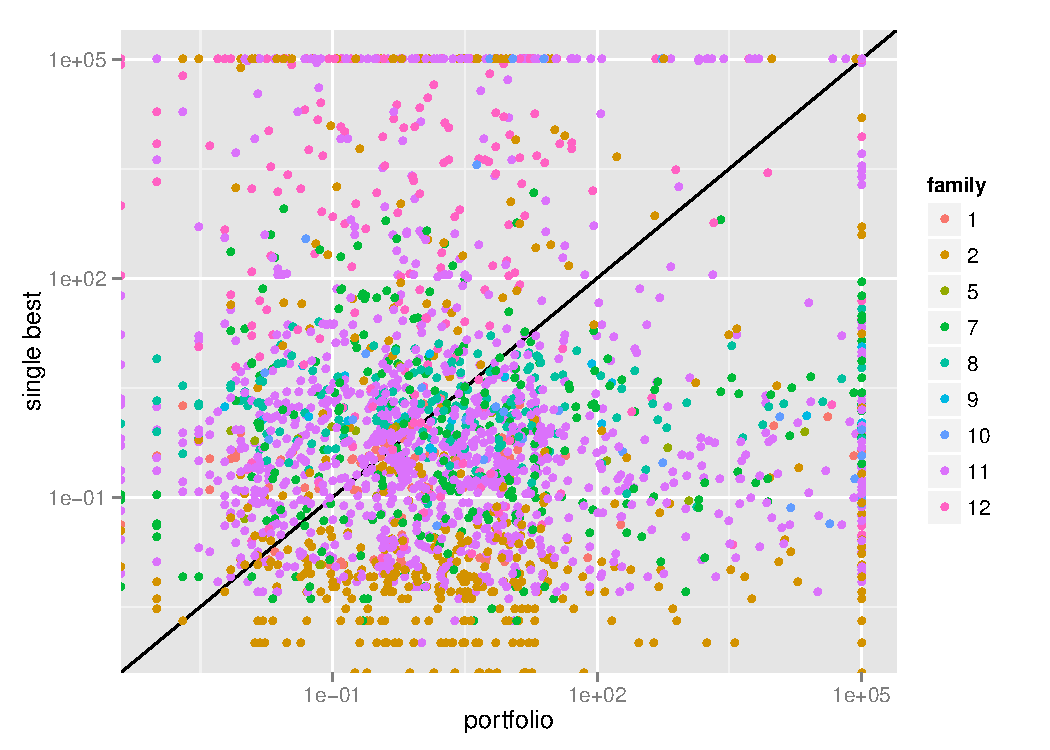
\includegraphics[width=\textwidth]{figures/perfScatter}
\caption{Single best algorithm vs.\ portfolio performance on all instances by
family. Points above the diagonal indicate that the portfolio achieved better
performance, while the single best solver was better on instances below the
diagonal.}
\label{fig:scatter}
\end{figure}

\section{Conclusion and Future Work}

This stuff works respectably well, considering we're dealing with two inputs rather than one.

We have only looked at sequential algorithms: the Glasgow algorithm has a parallel implementation,
and a similar technique could easily be used to parallelise LAD.  We have also not considered the
induced variant of the problem, nor instances involving labels or directed edges.  We could also
look at other encodings. For example, a direct SAT requires $O(v^4)$ clauses, but may be good in
certain situations.

\bibliographystyle{splncs}
\bibliography{paper}

\end{document}

